%---------------------------------------------------------------------
\begin{frame}{Recap on adverse selection}

    Health insurance: asymmetric information \& selection market\\
    \vspace{3mm}

    We have seen \newbold{two} models:
    \begin{enumerate}
        \item Einav and Finkelstein (2011): only premium varies across contracts
        {\color{white}\item[] Rothschild-Stiglitz (1976): both premium and level of insurance can vary across contracts}
    \end{enumerate}

\end{frame}
%---------------------------------------------------------------------
\begin{frame}{Einav and Finkelstein (2011) framework}

\begin{center}
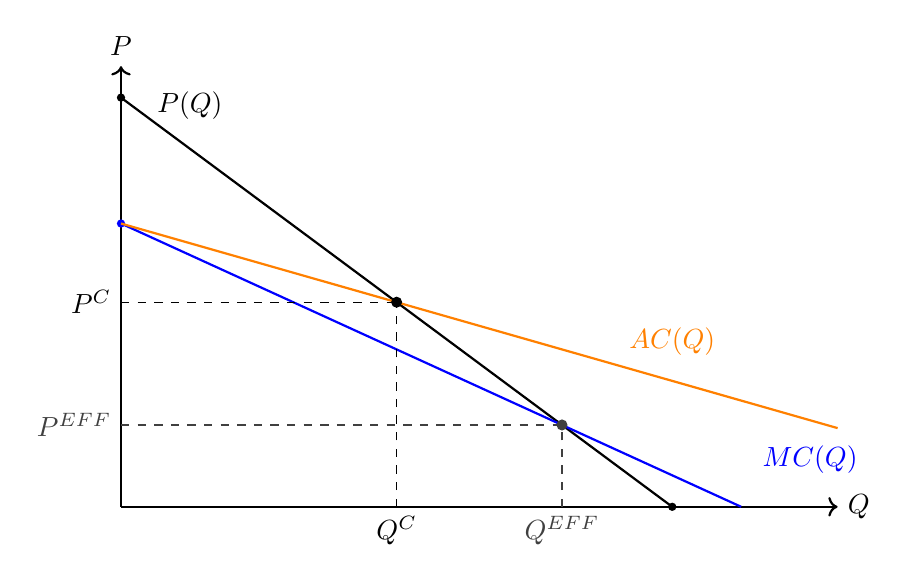
\begin{tikzpicture}[x=0.035cm, y=0.0020cm, scale=0.5]
\usetikzlibrary{arrows.meta}

    % Axes
    \draw[->, thick] (0,0) -- (520,0) node[right] {$Q$};
    \draw[->, thick] (0,0) -- (0,5600) node[above] {$P$};

    % Demand curve: P(Q) = 5200 - 13Q
    \draw[thick] (0,5200) -- (400,0);
    \node at (50,5100) {$P(Q)$};

    % Demand intercepts
    \fill (0,5200) circle[radius=3pt];
    \node[left] at (0,5200) {};

    \fill (400,0) circle[radius=3pt];
    \node[below] at (400,0) {};

    % ---- Marginal cost (lowered, same slope) ----
    % MC(Q) = 3600 - 8Q (x-intercept at Q=450)
    \draw[blue, thick] (0,3600) -- (450,0);
    \node[blue] at (500,600) {$MC(Q)$};

    \fill[blue] (0,3600) circle[radius=3pt];
    \node[left, blue] at (0,3600) {};

    % Average cost curve (lowered, same slope): AC(Q) = 3600 - 5Q
    \draw[orange, thick] (0,3600) -- (520,1000);
    \node[orange] at (400,2100) {$AC(Q)$};

    % Perfect competition equilibrium: intersection of Demand and AC
    % Solve: 5200-13Q = 3600-5Q  => 1600 = 8Q => Q=200, P=2600
    \fill (200,2600) circle[radius=4pt];
    \draw[dashed] (200,0) -- (200,2600);
    \draw[dashed] (0,2600) -- (200,2600);

    \node[below] at (200,0) {$Q^{C}$};
    \node[left] at (0,2600) {$P^{C}$};

    % ---- Efficient equilibrium: intersection of Demand and MC ----
    % Solve: 5200-13Q = 3600-8Q  => 1600 = 5Q => Q=320, P=1040
    \fill[darkgray] (320,1040) circle[radius=4pt];
    \draw[dashed, darkgray] (320,0) -- (320,1040);
    \draw[dashed, darkgray] (0,1040) -- (320,1040);

    \node[below, darkgray] at (320,0) {$Q^{EFF}$};
    \node[left,  darkgray] at (0,1040) {$P^{EFF}$};

\end{tikzpicture}
\end{center}

\end{frame}
%---------------------------------------------------------------------
\begin{frame}{Recap on adverse selection}

    Health insurance: asymmetric information \& selection market\\
    \vspace{3mm}

    We have seen \newbold{two} models:
    \begin{enumerate}
        \item Einav and Finkelstein (2011): only premium varies across contracts
        \item Rothschild-Stiglitz (1976): both premium and level of insurance can vary across contracts
    \end{enumerate}

\end{frame}
%---------------------------------------------------------------------
\begin{frame}{Rothschild-Stiglitz (1976) model}

    $(\Omega_1,\Omega_3)$ is a \newbold{separating equilibrium}
    \centering
    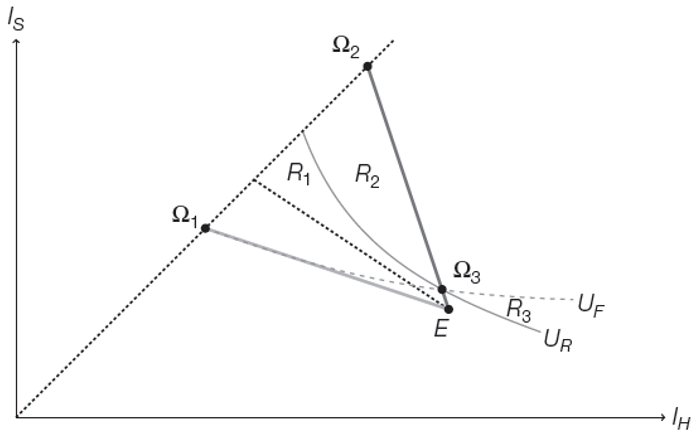
\includegraphics[width=0.8\textwidth]{./input/BHT_fig917.png}

\end{frame}
%---------------------------------------------------------------------
\begin{frame}{Why are these models useful?}

    Allowed us to think about
    \begin{itemize}
        \item Adverse selection and its impact on how many people get insured
        \pause
        \item Adverse selection and its impact on the bundle of insurance that people get
        \pause
        \item Whether unraveling occurs and under which conditions
        \pause
        % note two types of unraveling: the EF type or the RS type (mututally exclusive conceptually)
        \item Give us a framework to think about policy interventions (mandate, risk-adjustment, etc.)
        \pause
    \end{itemize}
    \vspace{3mm}

    We saw empirical evidence of
    \begin{itemize}
        \item Adverse selection
        \item Real world example of unraveling
    \end{itemize}

\end{frame}
%---------------------------------------------------------------------
\begin{frame}{Offered coverage in the real world}

    You are a policy maker and you notice that:
    \begin{itemize}
        \item Two identical plans are offered (same price, same coverage)
        \item Consumers choose plan randomly since the plans are identical\\
        $\implies$ no plan has a sicker pool of patients than the other
    \end{itemize}
    % It doesn't seem that adverse selection is a problem here, right?\\
    \pause
    \vspace{3mm}

    Now, you notice that both plans \textbf{do not cover chemotherapy drugs}.\\
    %Weird because consumers are probably willing to pay to insure themselves against the cost of getting cancer ==> inefficient 
    \pause
    \vspace{3mm}
    $\implies$ Based on your understanding of the Rothschild-Stiglitz model, what do you think is going on here?\\

\end{frame}
%---------------------------------------------------------------------
\begin{frame}{Offered coverage in the real world}

    You are a policy maker and you notice that:
    \begin{itemize}
        \item Two identical plans are offered (same price, same coverage)
        \item Consumers choose plan randomly since the plans are identical\\
        $\implies$ no plan has a sicker pool of patients than the other
    \end{itemize}
    % It doesn't seem that adverse selection is a problem here, right?\\
    \vspace{3mm}

    Now, you notice that both plans \textbf{do not cover chemotherapy drugs}.\\
    %Weird because consumers are probably willing to pay to insure themselves against the cost of getting cancer ==> inefficient 
    \vspace{3mm}
    $\implies$ Based on your understanding of the Rothschild-Stiglitz model, what do you think is going on here?\\
    \vspace{3mm}
    \newbold{Adverse selection is at play} here, influencing the equilibrium contract design.


\end{frame}
%---------------------------------------------------------------------
\begin{frame}{Contract features and risk adjustment}
\hypertarget{creamskimming}{}

    In the Rotschild-Stiglitz model,
    we see that insurers can compete using \newbold{contract features} (not just price) to attract different types of consumers.\\
    \hyperlink{RS:nopooling}{\beamerreturnbutton{Reminder from last class}}
    \vspace{3mm}
    %reminder on why no pooling

    Insurers can use contract features to attract different types of consumers
    \begin{itemize}
        \item Make contract less attractive to high-risk consumers (e.g. don't cover drugs they need)
        \item Make contract more attractive to low-risk consumers (e.g. gym membership, etc.)
    \end{itemize}
    \vspace{3mm}

    \only<2>{\textbf{What if we could intervene to remove these incentives for insurers?}}

\end{frame}
%---------------------------------------------------------------------
\begin{frame}{Example}

    The expected cost for a non-diabetic patient is \$5,000.\\
    Assume a patient with diabetes consumes \textbf{1.5 times} the amount of healthcare, in dollars, as a non-diabetic patient.\\
    Assume the premium is \$6,000 for both patients (the law prevents the insurer from charging different prices).\\
    \vspace{3mm}
    How much profit does the health insurer makes on each patient?
    \only<1>{
        \vspace{25mm}
    }
    \only<2>{
        \begin{itemize}
            \item For non-diabetic patient
            \begin{align*}
                E(\text{Profit}^{ND}) &= \text{premium} - E(\text{cost})\\
                &= 6000 - 5000 \\
                &= 1000
            \end{align*}
        \end{itemize}

    }
    \only<3>{
        \begin{itemize}
        \item For non-diabetic patient: $E(\text{Profit}^{ND}) = 1000$

        \item For diabetic patient:
        \begin{align*}
            E(\text{Profit}^{D}) &= \text{premium} - E(\text{cost}) + \text{subsidy}\\
            &= 6000 - 7500 \\
            &= -1500
        \end{align*}
        \end{itemize}
    }
    \only<4>{
        \begin{itemize}
        \item For non-diabetic patient: $E(\text{Profit}^{ND}) = 1000$

        \item For diabetic patient: $E(\text{Profit}^{D}) = -1500$
        \end{itemize}

        $\implies$ What are the incentives for this insurer?     
    }

\end{frame}
%---------------------------------------------------------------------
\begin{frame}{Example: introduce a government subsidy}

    The expected cost for a non-diabetic patient is \$5,000.\\
    Assume a patient with diabetes consumes 1.5 times the amount of healthcare, in dollars, as a non-diabetic patient.\\
    Assume the premium is \$6,000 for both patients (the law prevents you from charging different prices).\\
    \textbf{The government gives a subsidy of \$2,500 for each diabetic patient.}\\
    What are the incentives for the insurer now?
    \only<1>{
        \vspace{25mm}
    }
    \only<2>{
        \begin{itemize}
            \item For non-diabetic patient: $E(\text{Profit}^{ND}) = 1000$ (same)
            

            \item For diabetic patient:
            \vspace{-1mm}
            \begin{align*}
                E(\text{Profit}^{D}) &= \text{premium} - E(\text{cost}) + \text{subsidy}\\
                &= 6000 - 7500 + 2500 \\
                &= 1000
            \end{align*}
        \end{itemize}

    }
    \only<3>{
        \begin{itemize}
        \item For non-diabetic patient: $E(\text{Profit}^{ND}) = 1000$

        \item For diabetic patient: $E(\text{Profit}^{D}) = 1000$
        \end{itemize}

        $\implies$ The insurer does not care anymore which consumer it attracts!    
    }

\end{frame}
%---------------------------------------------------------------------
\begin{frame}{Risk-adjustment}

    \newbold{Risk-adjustment}: policy intervention to \textbf{remove incentives} for insurers to select on risk by adjusting payments to insurers based on the risk of their enrollees.\\
    The goal of the policy is to make the insurer indifferent between enrollees. How?\\
    $\implies$ By making insurers' \newbold{expected profit identical} across consumers.\\
    \vspace{3mm}

    Whom and how?
    \begin{itemize}
        \item Whom? Primarily managed by Centers for Medicare \& Medicaid Services (CMS)
        \item How? Hierarchical Condition Categories (HCCs) to map ICD-10 diagnosis codes to risk scores
    \end{itemize}

\end{frame}
%---------------------------------------------------------------------
\begin{frame}{Some examples of HCC coefficients }

    {\scriptsize
\begin{table}[htbp]
\centering
%\caption{CMS-HCC Relative Factors: Community, NonDual, Aged}
\begin{tabular}{llr}
\toprule
Group & Variable & Coefficient \\
\midrule
Female & 65--69 Years & 0.306 \\
Female & 70--74 Years & 0.368 \\
Female & 75--79 Years & 0.440 \\
Female & 80--84 Years & 0.528 \\
Female & 85--89 Years & 0.652 \\
Female & 90--94 Years & 0.783 \\
Female & 95 Years or Over & 0.802 \\
\midrule
Male & 65--69 Years & 0.295 \\
Male & 70--74 Years & 0.373 \\
Male & 75--79 Years & 0.458 \\
Male & 80--84 Years & 0.551 \\
Male & 85--89 Years & 0.682 \\
Male & 90--94 Years & 0.842 \\
Male & 95 Years or Over & 0.959 \\
\bottomrule
\end{tabular}
\end{table}
    }

    Source: \href{https://www.cms.gov/files/document/revised-cms-hcc-model-relative-factor-tablespdf}{CMS table}
    %CMS-HCC V22 2017-2023

\end{frame}
%---------------------------------------------------------------------
\begin{frame}{Some examples of HCC coefficients}

    {\scriptsize
\begin{table}[htbp]
\centering
%\caption{CMS-HCC Disease Coefficients: Community, NonDual, Aged}
\begin{tabular}{llr}
\toprule
HCC & Description & Coefficient \\
\midrule
HCC1 & HIV/AIDS & 0.306 \\
%HCC2 & Septicemia, Sepsis, Systemic Inflammatory Response Syndrome/Shock & 0.447 \\
HCC6 & Opportunistic Infections & 0.428 \\
HCC8 & Metastatic Cancer and Acute Leukemia & 2.579 \\
HCC9 & Lung and Other Severe Cancers & 0.953 \\
HCC17 & Diabetes with Acute Complications & 0.312 \\
HCC19 & Diabetes without Complication & 0.102 \\
HCC22 & Morbid Obesity & 0.268 \\
HCC27 & End-Stage Liver Disease & 0.945 \\
HCC28 & Cirrhosis of Liver & 0.383 \\
HCC47 & Disorders of Immunity & 0.614 \\
HCC57 & Schizophrenia & 0.597 \\
HCC58 & Major Depressive, Bipolar, and Paranoid Disorders & 0.388 \\
%HCC70 & Quadriplegia & 1.291 \\
HCC71 & Paraplegia & 0.989 \\
HCC77 & Multiple Sclerosis & 0.434 \\
HCC78 & Parkinson's and Huntington's Diseases & 0.662 \\
%HCC80 & Coma, Brain Compression/Anoxic Damage & 0.574 \\
\bottomrule
\end{tabular}
\end{table}
    }
    Source: \href{https://www.cms.gov/files/document/revised-cms-hcc-model-relative-factor-tablespdf}{CMS table}
    %CMS-HCC V22 2017-2023

\end{frame}
%---------------------------------------------------------------------
\begin{frame}{Mechanics of risk-adjustment}

    The insurer receives a payment $R_i$ for each enrollee $i$ based on the risk of that enrollee.
    It is calculated as 
    \begin{align*}
        R_i = \phi \cdot r_i
    \end{align*}
    \vspace{-2mm}
    where
    \begin{enumerate}
        \item $\phi$ is a benchmark payment for all enrollees (for example, \$800 per month)
        \item $r_i$ is the risk score of enrollee $i$, which is calculated based on a set of risk adjusters $x_i$.
        \begin{align*}
            r_i = \sum \lambda x_i
        \end{align*}
        where $x_i$ are typically indicators for a small set of chronic conditions, and $\lambda$ is a set of coefficients to weight each risk adjuster.\\
        Note: not all risk-adjusters are weighted the same 
        %$\implies$ $\lambda$ is a set of coefficients that varies across risk adjusters.
    \end{enumerate}

\end{frame}
%---------------------------------------------------------------------
\begin{frame}{Risk-adjustment: example}

    Assume the benchmark payment $\phi$ is \$800 per month. \\
    The risk score includes an indicator for diabetes and for huntington disease.\\
    The weight for diabetes is $\lambda_{diabetes} = 1.5$ and the weight for huntington disease is $\lambda_{huntington} = 2.5$.\\
    Consider three enrollees:
    \only<1>{
    \begin{itemize}
        \item Enrollee 1 has diabetes but not huntington disease
        \item Enrollee 2 has huntington disease but not diabetes
        \item Enrollee 3 has neither diabetes nor huntington disease
    \end{itemize}
    \vspace{3mm}
    What payment does the insurer receive for each enrollee?

        \vspace{10mm}
    }

    \only<2>{
        \begin{itemize}
            \item Enrollee 1 (diabetes only): $R_1 = 800 \cdot (1.5 \cdot 1 + 2.5 \cdot 0) = 1200$
            \item Enrollee 2 (huntington disease only): $R_2 = 800 \cdot (1.5 \cdot 0 + 2.5 \cdot 1) = 2000$
            \item Enrollee 3 (neither): $R_3 = 800 \cdot (1.5 \cdot 0 + 2.5 \cdot 0) = 0$
        \end{itemize}
    }

    \only<3>{
        \begin{itemize}
            \item Enrollee 1 (diabetes only): $R_1 = 800 \cdot (1.5 \cdot 1 + 2.5 \cdot 0) = 1200$
            \item Enrollee 2 (huntington disease only): $R_2 = 800 \cdot (1.5 \cdot 0 + 2.5 \cdot 1) = 2000$
            \item Enrollee 3 (neither): $R_3 = 800 \cdot (1.5 \cdot 0 + 2.5 \cdot 0) = 0$
        \end{itemize}

        Why did the government set the weights $\lambda$ this way?\\
        $\implies$ The government set the weights to reflect the expected cost of each condition.
    }

\end{frame}
%---------------------------------------------------------------------
\begin{frame}{Risk-adjustment and \textit{expected} health differences}

    The risk-adjustment payment is based on \textit{expected} health differences across enrollees.\\
    $\implies$ What about high-variance conditions?\\
    \pause
    For example, two enrollees may have the same expected cost, but one enrollee may have a much higher variance in cost than the other enrollee:
    \begin{itemize}
        \item Enrollee 1: cost is \$10,000 for sure
        %expected is 10,000 with variance of 0
        \item Enrollee 2: 90\% chance of \$0 and 10\% chance of \$100,000
        %expected is 10,000 with variance of 900,000,000
    \end{itemize}
    \vspace{3mm}

    Solution? 
    \pause \newbold{Reinsurance}


\end{frame}
%---------------------------------------------------------------------
\begin{frame}{Reinsurance}

    \newbold{Reinsurance}: insurance for insurers to protect them from high-cost enrollees.\\
    $\implies$ Could be sold to insurers and/or provided by government.\\
    \vspace{3mm}

    How does it work?\\
    \begin{itemize}
    \item The insurer pays a premium to a reinsurer.
    \item If claims exceed a threshold, the reinsurer reimburses part of the losses.
    \end{itemize}

\end{frame}
%---------------------------------------------------------------------
\begin{frame}{Reinsurance example}

    Example in the ACA (2014 parameters):
    \begin{align*}
        \text{Reinsurance payment} = \gamma \times max\{0, \text{enrollee cost} - \text{attachment point}\}
    \end{align*}
    where
    \begin{itemize}
        \item $\gamma$ is the coinsurance rate: set to 80\%
        \item The attachment point is \$45,000
        \item There is usually a cap: \$250,000
    \end{itemize}

\end{frame}
%---------------------------------------------------------------------
\begin{frame}{Reinsurance example}

    \begin{align*}
        \text{Reinsurance payment} = 0.8 \times max\{0, \text{enrollee cost} - 45,000\}
    \end{align*}
    + cap of \$250,000\\
    \vspace{3mm}

    \only<1>{
        What is the enrollee ends up costing \$100,000?
        \vspace{25mm}
    }
    \only<2>{
        What is the enrollee ends up costing \$100,000?
        \begin{align*}
            \text{Reinsurance payment} &= 0.8 \times max\{0, 100,000 - 45,000\} \\
            &= 0.8 \times 55,000 \\
            &= 44,000
        \end{align*}
    }
    \only<3>{
        What if the enrollee ends up costing \$400,000?
        \begin{align*}
            \text{Reinsurance payment} &= 0.8 \times max\{0, 400,000 - 45,000\} \\
            &= 0.8 \times 355,000 \\
            &= 284,000
        \end{align*}
        But there is a cap of \$250,000, so the reinsurance payment is \$250,000.
    }

\end{frame}
%---------------------------------------------------------------------
\begin{frame}{Summary}

    Risk-adjustment and reinsurance both aim to remove incentives for insurers to select on risk.\\
    \begin{itemize}
        \item Risk-adjustment: \textit{expected} health differences across enrollees
        \item Reinsurance: \textit{high-variance} or high-tail risk enrollees
    \end{itemize}    
    \vspace{3mm}

    Note that risk-adjustment and reinsurance most likely influence the \textbf{intensive margin} of insurance (how much insurance you get when you get it)
\end{frame}
%---------------------------------------------------------------------
\begin{frame}{In practice?}

    All of this has been theory so far
    \begin{itemize}
        \item Do you think insurers are sophisticated enough to do this?
        \pause
        \item Do the risk-adjustment systems that exist (e.g. the one from the ACA) work as intended?
    \end{itemize}
    \pause
    \vspace{5mm}

    Let's look at the research!

 
\end{frame}
%---------------------------------------------------------------------
\begin{frame}{Geruso, Layton, and Prinz (2019)}

\centering
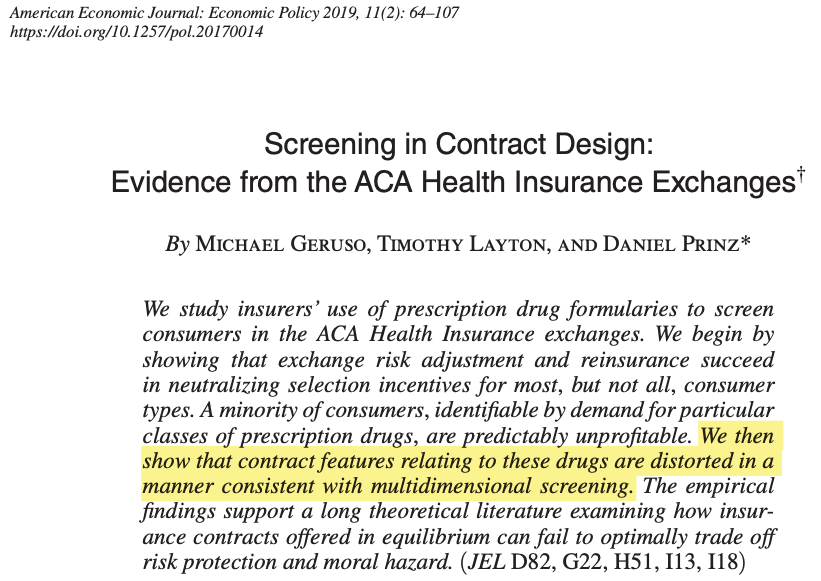
\includegraphics[width=0.75\textwidth]{input/GLP_front.png}
 
\end{frame}
%---------------------------------------------------------------------
\begin{frame}{Geruso, Layton, and Prinz (2019) - context}

    The patient Protection and Affordable Care Act (ACA) of 2010
    \begin{itemize}
        \item Created the Marketplace for individual health insurance
        \item Payment adjustments: risk-adjustment and reinsurance programs (2014 - 2016)
    \end{itemize}
    \vspace{3mm}

    Look at \newbold{prescription drug benefits}, i.e. which drugs are covered by insurance plans and how much they are covered (drug formularies)


\end{frame}
%---------------------------------------------------------------------
\begin{frame}{Risk-adjustment incentives}

    \newbold{Idea 1}: risk-adjustment should have eliminated incentives for insurers to select on risk across drug classes within plan...\\
    \pause
    but it may not be perfect: ``adjustment errors''\\
    \pause
    \vspace{5mm}

    How to check this?
    %You want to compare the cost of people who take a drug against the revenue the insurer made from them, after receiving risk-adjustment payments

\end{frame}
%---------------------------------------------------------------------
\begin{frame}{Risk-adjustment incentives across drug classes}

    You want to compare across \textbf{drug classes}
    \begin{itemize}
        \item The average medical expense of people who took a drug class in a year
        \item The revenue from an insurer with an \textit{actuarially fair premium} + risk-adjustment payments (expected actuarially fair insurer revenue)
    \end{itemize}
    \vspace{5mm}

    If risk-adjustment is successful, what do you expect to see?
    %Expected cost = expected revenue so that on 45 degree line

    % Note that it is not easy, you need to map each drug to a drug class first.
    
\end{frame}
%---------------------------------------------------------------------
\begin{frame}{Risk-adjustment incentives in picture}

    \centering
    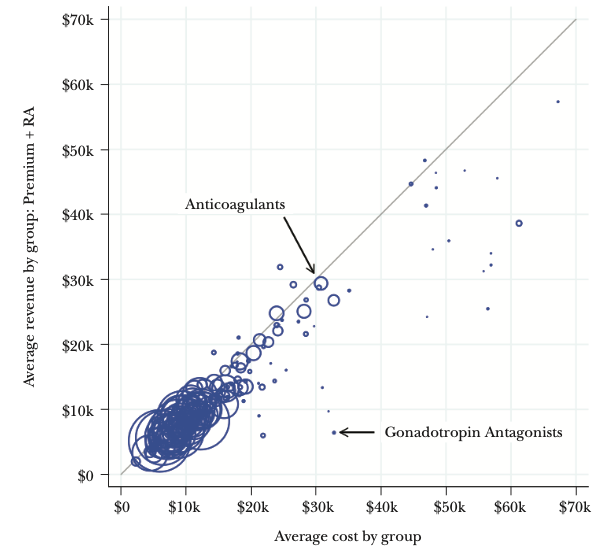
\includegraphics[width=0.6\textwidth]{input/GL_fig5.png}

\end{frame}
%---------------------------------------------------------------------
\begin{frame}{Risk-adjustment incentives in picture}

    \begin{columns}
        \begin{column}{0.6\textwidth}
            \vspace{-1mm}
            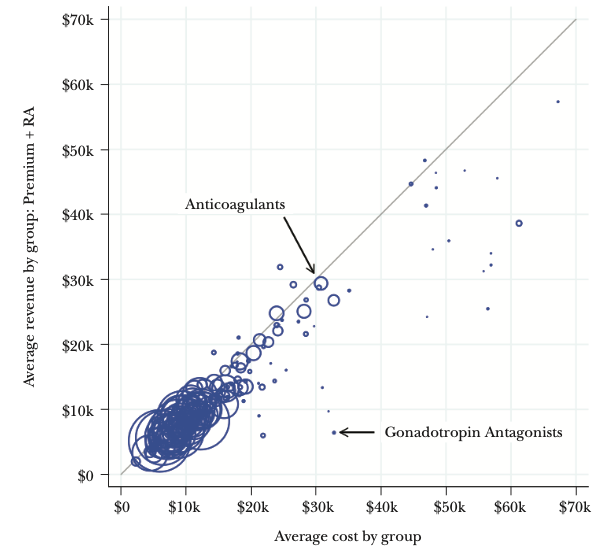
\includegraphics[height=0.9\textheight]{input/GL_fig5.png}
        \end{column}
        \begin{column}{0.4\textwidth}
            Notice that
            \begin{itemize}
                \item The points are close to the 45 degree line: risk-adjustment is successful
                \item BUT there is some variation across drug classes: risk-adjustment is not perfect
            \end{itemize}
        \end{column}
    \end{columns}

\end{frame}
%---------------------------------------------------------------------
\begin{frame}{Incentives vary between exchange and self-insured plans}

    \newbold{Idea 2}: compare drug formularies in plans
    \begin{itemize}
        \item Exchange plans (on the Marketplace)
        \item Self-insured employer plans
    \end{itemize}
     Why? Because incentives to ``cream-skim'' are different in self-insured plans.\\
    \textit{Do you see why?}
    % Self-insured employers: do not change the pool of insurees, they need to insure everyone
    \pause
    \vspace{5mm}

    Let's see what it looks like in the data!\\
    \pause
    \textit{How?}
    % Let's see if drugs are more restrcited in exchange plans

\end{frame}
%---------------------------------------------------------------------
\begin{frame}{Drug classes are more likely to be restricted in exchange plans}

    \centering
    \only<1>{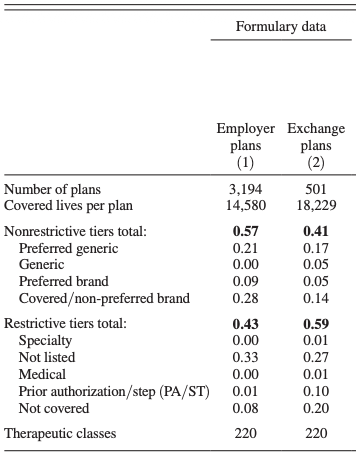
\includegraphics[width=0.4\textwidth]{input/GLP_tab1.png}}
    \only<2>{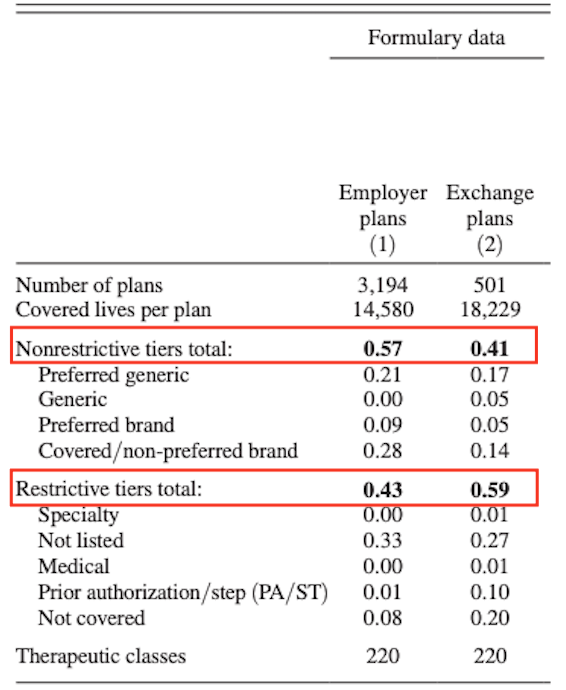
\includegraphics[width=0.4\textwidth]{input/GLP_tab1H.png}}

\end{frame}
%---------------------------------------------------------------------
\begin{frame}{Geruso, Layton, and Prinz (2019) - empirical strategy}

    You have \textbf{two} levels of difference: \newbold{difference-in-difference} approach
    \vspace{5mm}

    They compare drug formularies in
    \begin{itemize}
        \item Exchange plans vs self-insured employer plans
        \item Between drug classes within plans
    \end{itemize}

\end{frame}
%---------------------------------------------------------------------
\begin{frame}{Geruso, Layton, and Prinz (2019) - results in a picture}

    \centering
    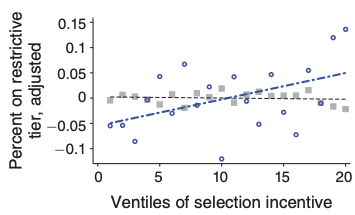
\includegraphics[width=0.7\textwidth]{input/GLP_fig5b.png}
    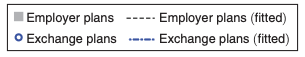
\includegraphics[width=0.6\textwidth]{input/GLP_fig5blegend.png}

    % 20 groups of selection incentives: from low to high
    % When employer plan: flat
    % When exchange plan: more likely to be restricted when selection incentives are higher

\end{frame}
%---------------------------------------------------------------------
\begin{frame}{Geruso, Layton, and Prinz (2019) - summary}

    Key contributions:
    \begin{enumerate}
        \item Risk-adjustment and reinsurance are successful at smoothing incentives in the ACA
        \item Show empirically that drug formularies are responsive to selection incentives
    \end{enumerate}
    \vspace{5mm}

    Empirical strategy: difference-in-difference
    \begin{itemize}
        \item Variation across drug classes within plan
        \item Variation for self-insured versus exchange plans
    \end{itemize}

\end{frame}
%---------------------------------------------------------------------
\begin{frame}{More on risk-adjustment}

    Risk-adjustment is hard to do well in practice!
    \begin{itemize}
        \item It will be imperfect
        \item Can create new incentives 
        \begin{itemize}
            \item Eliminate some incentives but create others
            \item \newbold{Upcoding}: coding more \textit{profitable} diagnoses to get higher risk-adjustment payments for the same patient\\
            $\implies$ This is shown in the research from Geruso and Layton (2020) ``Upcoding: Evidence from Medicare on Squishy Risk Adjustment''
        \end{itemize}
    \end{itemize}

\end{frame}
%---------------------------------------------------------------------
\begin{frame}{Summary of policy intervention}

    You now have the tools to understand the source and consequences of policy interventions in health insurance markets.\\
    \vspace{3mm}
    \pause

    \begin{itemize}
        \item \newbold{Premium rating (or ``Community ratings'')}: prevents insurers from charging different prices to different consumers based on their risk\\
        \pause
        $\implies$ Exacerbates adverse selection by creating an information asymmetry
        \item \newbold{Mandate}: forces everyone to buy insurance\\
        \pause
        $\implies$ Can help mitigate adverse selection by ensuring a larger and more diverse risk pool (extensive margin)
        %This will influence the extensive margin on how many people are insured
        \pause
        \item \newbold{Risk-adjustment \& reinsurance}: adjusts payments to insurers based on the risk of their enrollees + insuring them against high cost events\\
        \pause
        $\implies$ Can help mitigate adverse selection by removing incentives for insurers to select on risk (intensive margin)
        % This will help the intensive margin of how much insurance you get when you get it
    \end{itemize}
 
\end{frame}
%---------------------------------------------------------------------
\begin{frame}{(Highly) Recommended reading}

    Geruso \& Layton (2017) ``Selection in Health Insurance Markets and Its Policy Remedies''
    in the \textit{Journal of Economic Perspectives}\\
    (posted on Blackboard)

    
 
\end{frame}
%---------------------------------------------------------------------
\begin{frame}{}
    \begin{center}
    \Large \textcolor{maroon}{Wrapping up}
    \end{center}
\end{frame}
%---------------------------------------------------------------------
\begin{frame}{To next class}
\begin{itemize}
    \item \newbold{TO DO}
    \begin{enumerate}
        \item Review this class and past material $\implies$ \textit{questions on it?}
        \item \newbold{Mandatory READING 2}: Chapter 1 of Gross and Notowidigdo's book \textit{Better Health Economics} (posted on Blackboard)
    \end{enumerate}
    \vspace{5mm}

    \item Program for next class
    \begin{itemize}
        \item What does health insurance do?
    \end{itemize}
\end{itemize}
\end{frame}
%---------------------------------------------------------------------